
%(BEGIN_QUESTION)
% Copyright 2010, Tony R. Kuphaldt, released under the Creative Commons Attribution License (v 1.0)
% This means you may do almost anything with this work of mine, so long as you give me proper credit

Suppose we have a Siemens S7-200 PLC connected to a pair of pushbutton switches and light bulbs as shown in this illustration:

$$\includegraphics[width=15.5cm]{i04630x01.eps}$$

Examine the following relay ladder logic (RLL) program for this Siemens PLC, determining the statuses of the two lamps provided neither switch is pressed by a human operator:

$$\includegraphics[width=15.5cm]{i04630x02.eps}$$

\underbar{file i04630}
%(END_QUESTION)





%(BEGIN_ANSWER)

Output {\tt Q0.1} will activate to energize lamp Y, but the other output (and lamp) will remain off. 

%(END_ANSWER)





%(BEGIN_NOTES)


%INDEX% PLC, relating I/O status to virtual elements

%(END_NOTES)


